\documentclass[main.tex]{subfiles}
\begin{document}

\section{Draw a circuit to control a green LED from a microcontroller GPIO pin.}

It is desired to operate the LED at a forward current of 10mA. Assume that the LED has a forward voltage drop of 2V at the desired forward current. The microcontroller GPIO pin can source a maximum of 5mA, and operates at 3.3V.

\spoilerline
\subsection{Context}
Discrete LEDs (\textit{Light Emitting Diodes}) are often used on circuit boards indicators to end users and firmware developers about the state of an embedded system\footnote{LEDs can also be a primary feature of a device - an example case is high power LEDs, such as automobile headlights, which require more complex circuitry to drive. This question will address only the simpler case of lower power LEDs.}. A common first program executed during board bring-up by firmware developers is to blink the onboard LEDs as an indicator the microcontroller is alive and functional. For end users, it is very common to use LEDs to indicate that the embedded system is powered on and operating nominally. Often, in electronic circuits, an LED is connected in some fashion to a microcontroller GPIO (\textit{General Purpose Input / Output}) pin in order to turn it on and off via firmware. 

\subsection{Controlling Current to an LED} 
\noindent The circuit given in Figure \ref{fig:led_circuit_simple} shows a schematic of an LED powered from a constant voltage source, $V_s$, with a fixed resistance, $R_l$ in series with the LED. Note this circuit cannot be controlled by a microcontroller yet. The LED has a forward voltage drop, $V_f$, and a forward current, $I_f$. The goal is to determine the value of $R_l$, limiting the current through the LED ($I_f$).

\begin{figure}[h!]
    \begin{center}
        \begin{circuitikz}[american]
            \draw (0, 6) node[vcc] () {$V_s$};
            \draw (0, 6) to[empty led, v=$V_f$, i=$I_f$] (0, 4);
            \draw (0, 4) to[resistor, l=$R_l$] (0, 2);
            \draw (0, 2) node[ground] () {};
            \label{fig:led_circuit_simple}
        \end{circuitikz}
        \caption{Voltage Source Powering an LED}
    \end{center}
\end{figure}

\noindent The circuit can be solved by modelling the forward voltage drop of the LED, $V_f$, as a fixed voltage and applying Ohms Law to solve for solve for $R_l$, as shown in equation \eqref{eq:led_current_limitting_resistor_math}:

\begin{equation}
    \begin{aligned}[b]
        V_s - V_f &= R_l \cdot I _f \\
        R_l &= \frac{V_s - V_f}{I_f}
    \end{aligned}
    \label{eq:led_current_limitting_resistor_math}
\end{equation}

\noindent Note that for LEDs, the brightness is roughly proportional to the current flowing through the LED. Consequently, the brightness of the LED can be varied by changing the resistance value or the voltage to the LED\footnote{To give a reference, a small, surface-mounted LED are usually rated for 20mA max (so 20mA * 2V = 40mW), and are visible indoors at just 1mA. For a firmware debugging LED, ~2.5mA, is very common}. In practice, an LED's forward voltage is somewhat dependent on $I_f$ and device temperature. "I-V Curves" across temperature are usually given by LED manufacturers in the LED's datasheets, however, an assumption of a constant $V_f$ is enough for approximate solutions.

\subsection{Transistors}
Transistors are three terminal, electronically-controlled switches in which one terminal is used to control the switching between the other two terminals. The two most commonly used transistors are MOSFETs (\textit{Metal Oxide Semiconductor Field Effect Transistors}) and BJTs (\textit{Bipolar Junction Transistors}), though there are other types. For a BJT, a small current to the base allows a large current to flow between emitter and collector terminals. For a FET (\textit{Field Effect Transistor}), a voltage potential difference between the gate and the source allows current to flow between drain and source. These devices can be drawn with a variety of schematic symbols, but are most commonly seen as:

\begin{figure}[H]
    \begin{center}
        \begin{circuitikz}[american]
            \draw (0, 4) node[npn] (q1) {NPN BJT};
            \draw (q1.E) ++ (0, -0.5) node[anchor=south]{Emitter};
            \draw (q1.B) ++ (-1, 0) node[anchor=west]{Base};
            \draw (q1.C) ++ (0, 0.5) node[anchor=north]{Collector};
            \draw (4, 4) node[pnp] (q2) {PNP BJT};
            \draw (q2.E) ++ (0, 0.5) node[anchor=north]{Emitter};
            \draw (q2.B) ++ (-1, 0) node[anchor=west]{Base};
            \draw (q2.C) ++ (0, -0.5) node[anchor=south]{Collector};
            \draw (8, 4) node[nigfete](q3){NCH FET};
            \draw (q3.G) ++ (-1, 0) node[anchor=west]{Gate};
            \draw (q3.S) ++ (0, -0.5) node[anchor=south]{Source};
            \draw (q3.D) ++ (0, 0.5) node[anchor=north]{Drain};
            \draw(12, 4) node[pigfete](q4){PCH FET};
            \draw (q4.G) ++ (-1, 0) node[anchor=west]{Gate};
            \draw (q4.D) ++ (0, -0.5) node[anchor=south]{Drain};
            \draw (q4.S) ++ (0, 0.5) node[anchor=north]{Source};
            \label{fig:transistors}
        \end{circuitikz}
        \caption{Common Transistors}
    \end{center}
\end{figure}

\noindent FETs, ideally, do not require any power consumption to keep them enabled, whereas BJTs require current to be supplied constantly. This means FETs are typically preferred when power consumption is a critical consideration; this is primarily for higher power circuits in which excessive power consumption directly results in a need for expensive cooling systems. BJTs are a much older technology and are easier to fabricate, making them far preferred when optimizing for cost. \newline

Another consideration is low side switching vs high side switching when using a transistor to enable and disable (aka switch) a load. The solution given in Figure \ref{fig:led_circuit} demonstrates low side switching. There are numerous implications of this design decision that are out of the scope of this guide.
% Trying to avoid scope creep here. This concept is not covered further at all in this guide, saving for second edition lol.

\subsection{Controlling the LED from a Microcontroller}

\noindent The microcontroller GPIO (\textit{General Purpose Input / Output}) pin is not capable of providing enough current to drive the LED (\textit{Light Emitting Diode}) as desired so an external transistor is required to buffer the signal from the microcontroller. The following circuit in Figure \ref{fig:led_circuit} demonstrates a simple cost optimized solution to this question. 

\begin{figure}[h!]
    \begin{center}
        \begin{circuitikz}[american]
            \draw (0, 6) node[vcc] () {$+3.3V$};
            \draw (0, 6) to[empty led] (0, 4.5);
            \draw (0, 4.5) to[resistor, l=$R_l$] (0, 3);
            \draw (0, 3) -- (0, 2.5);
            \draw (0, 2) node[npn, xscale=-1] (q1) {};
            \draw (q1.E) node[ground]{};
            \draw (q1.B) to[resistor, l=$R_b$] ++ (2.2, 0);
            \draw[thick] (3, 3) rectangle (5, 1) node[pos=0.5]{GPIO};
            \label{fig:led_circuit}
        \end{circuitikz}
        \caption{GPIO driving an LED}
    \end{center}
\end{figure}

An NPN BJT is used to switch the LED on and off. This type of transistor is defined by: $I_C = I_B \cdot \beta$, $V_{BE} \approx 0.7 V$, and $\beta \approx 100$. Note that these are approximations and vary based on the part number selected. $I_C$ represents current into the collector pin, $I_B$ represents current into the base pin, current out of the emitter, $I_E$, is given by $I_E = I_B + I_C$, and $V_{BE}$ is the forward voltage drop from the base to the emitter. When the GPIO is low, $V_{gpio} = 0$, $V_b \approx V_e = 0$, therefore $I_b = I_c = 0$ and consequently the LED is off. When the GPIO is high, $V_{gpio} = V_{logic-high} = 3.3V$, the desired behavior is to enable the transistor as much as possible, $V_c \approx 0V$. To provide some margin on the GPIO  current limit at $I_{b_{max}} = 5 mA$ the target current could be $I_b \approx \frac{I_{b_{max}}}{2} = 2.5mA$. This is acceptable as $I_c = I_b \cdot \beta = 2.5mA \cdot 100 = 250mA >> 10mA$ where 10mA is going to be the current limit enforced by the value of $R_l$. The intended $I_b$ can be used to solve for $R_b$ using Ohm's Law where $V_{gpio} - V_{b} = I_b \cdot R_b$. Because for this circuit $V_{b} = V_{be}$ the equation becomes $R_b = \frac{V_{gpio} - V_{b}}{I_b} = \frac{3.3V-0.7V}{2.5mA} = 1040 \Omega$. To round to commonly available resistor values gives  $R_b = 1 k \Omega$ as a reasonable solution.

The forward voltage drop of a green LED, $V_f$, is roughly 2 V so Ohms law can be used to solve for the value of $R_l$. Ohms Law gives $\frac{V_s - V_f} = I_f \cdot R_l$ which can be rearranged into $R_l = \frac{V_s - V_f}{I_f} = \frac{3.3V-2V}{10m} = 130 \Omega$. This resistor can be found in the E24 resistor series as a common resistor value so no rounding is needed. 

\subsection{Pulse Width Modulation}
When controlling an LED from a microcontroller, the brightness of the LED can be modulated using PWM (\textit{Pulse Width Modulation}). Adjusting the \textit{duty cycle} (amount of 'on' or logic high time) of pulse width modulation, provided the frequency $f$ is much greater than perceivable by the human eye, results in the appearance that the LED brightness is changing. If $f$ is too low then it will be apparent to a viewer that the LED is turning on and off. PWM implementations are usually done in hardware via dedicated timers, where the frequency is set to a constant, high value and the timer's duty cycle is adjusted to control the brightness. An example of a PWM waveform with a duty cycle of 80\% is shown in figure \ref{fig:pwm_waveform}.

\begin{figure}[H]
    \centering
    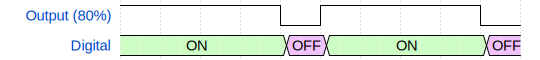
\includegraphics[scale=0.4]{generated_images/svg_generated/pwm.png}
    \caption{PWM Waveform}
    \label{fig:pwm_waveform}
\end{figure}

\noindent Note that PWM's application is not limited to LEDs - in general, PWM can be thought of as a way to control the average voltage across a load, and is used in motor control, power supplies, and more.

\end{document}
